%!TEX TS-program = pdflatexmk

% Copyright (c) 2018 - 2022, Martin Scheidt (ISC license)
% Permission to use, copy, modify, and/or distribute this file for any purpose with or without fee is hereby granted, provided that the above copyright notice and this permission notice appear in all copies.

\documentclass[border=2]{standalone}

\usepackage{siunitx}
\sisetup{
  text-family-to-math = true,
  text-series-to-math = true
}
\usepackage[prefix=]{xcolor-solarized}

\usepackage[dev]{tikz-trackschematic}

\begin{document}
  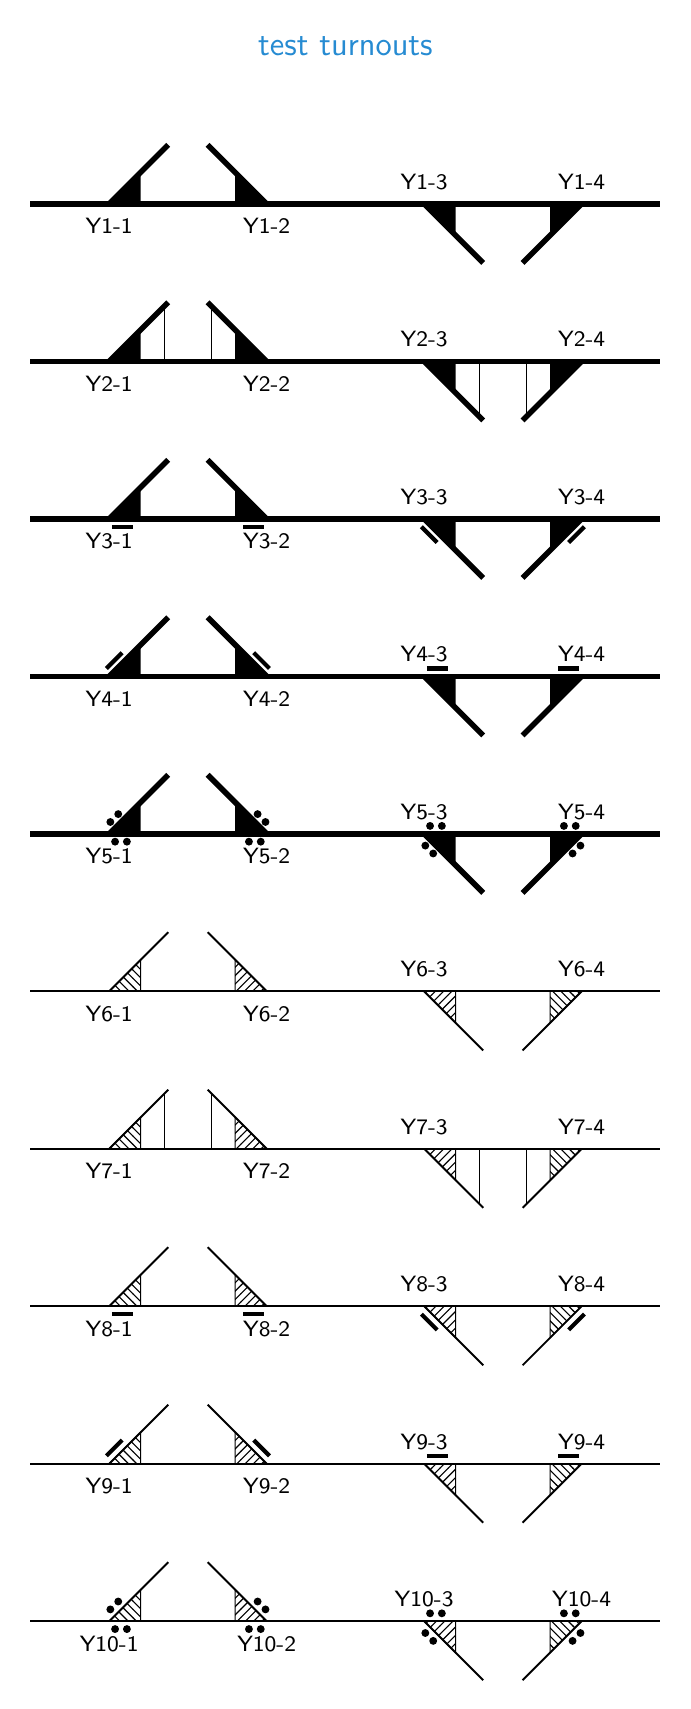
\begin{tikzpicture}[font=\sffamily]
    %!TEX TS-program = pdflatexmk
%!TEX root = test.tex

% Copyright (c) 2018 - 2021, Martin Scheidt (ISC license)
% Permission to use, copy, modify, and/or distribute this file for any purpose with or without fee is hereby granted, provided that the above copyright notice and this permission notice appear in all copies.

\node[blue] at (4,0) {\large test turnouts};

\foreach \i in {1,2,...,10}{% base coordinate
  \coordinate (A\i) at ($(0,0) + 2*(0,-\i)$);
  \coordinate (B\i) at ($(8,0) + 2*(0,-\i)$);
}

\foreach \i in {1,2,...,5}{% draw main tracks on base coordinate
  \maintrack (A\i) --   (B\i);
}

\foreach \i in {6,7,...,10}{% draw secondary tracks on base coordinate
  \secondarytrack (A\i) --   (B\i);
}

\foreach \i in {1,2,...,10}{% coordinates for testing symbols
  \coordinate (Y\i-1) at ($(1,0) + 2*(0,-\i)$);
  \coordinate (Y\i-2) at ($(3,0) + 2*(0,-\i)$);
  \coordinate (Y\i-3) at ($(5,0) + 2*(0,-\i)$);
  \coordinate (Y\i-4) at ($(7,0) + 2*(0,-\i)$);
}

\foreach \i in {1,2,...,5}{% coordinates for testing symbols
  \maintrack  (Y\i-1) -- ++( 0.75, 0.75);
  \maintrack  (Y\i-2) -- ++(-0.75, 0.75);
  \maintrack  (Y\i-3) -- ++( 0.75,-0.75);
  \maintrack  (Y\i-4) -- ++(-0.75,-0.75);
}

\foreach \i in {6,7,...,10}{% coordinates for testing symbols
  \secondarytrack  (Y\i-1) -- ++( 0.75, 0.75);
  \secondarytrack  (Y\i-2) -- ++(-0.75, 0.75);
  \secondarytrack  (Y\i-3) -- ++( 0.75,-0.75);
  \secondarytrack  (Y\i-4) -- ++(-0.75,-0.75);
}

\turnout[forward ,branch=left ] at (Y1-1) label (Y1-1);
\turnout[backward,branch=left ] at (Y1-2) label (Y1-2);
\turnout[forward ,branch=right] at (Y1-3) label (Y1-3);
\turnout[backward,branch=right] at (Y1-4) label (Y1-4);
\turnout[forward ,branch=left ,fouling point] at (Y2-1) label (Y2-1);
\turnout[backward,branch=left ,fouling point] at (Y2-2) label (Y2-2);
\turnout[forward ,branch=right,fouling point] at (Y2-3) label (Y2-3);
\turnout[backward,branch=right,fouling point] at (Y2-4) label (Y2-4);
\turnout[forward ,branch=left ,points=right] at (Y3-1) label (Y3-1);
\turnout[backward,branch=left ,points=right] at (Y3-2) label (Y3-2);
\turnout[forward ,branch=right,points=right] at (Y3-3) label (Y3-3);
\turnout[backward,branch=right,points=right] at (Y3-4) label (Y3-4);
\turnout[forward ,branch=left ,points=left ] at (Y4-1) label (Y4-1);
\turnout[backward,branch=left ,points=left ] at (Y4-2) label (Y4-2);
\turnout[forward ,branch=right,points=left ] at (Y4-3) label (Y4-3);
\turnout[backward,branch=right,points=left ] at (Y4-4) label (Y4-4);
\turnout[forward ,branch=left ,points=moving] at (Y5-1) label (Y5-1);
\turnout[backward,branch=left ,points=moving] at (Y5-2) label (Y5-2);
\turnout[forward ,branch=right,points=moving] at (Y5-3) label (Y5-3);
\turnout[backward,branch=right,points=moving] at (Y5-4) label (Y5-4);

\turnout[forward ,branch=left ,operation=manual] at (Y6-1) label (Y6-1);
\turnout[backward,branch=left ,operation=manual] at (Y6-2) label (Y6-2);
\turnout[forward ,branch=right,operation=manual] at (Y6-3) label (Y6-3);
\turnout[backward,branch=right,operation=manual] at (Y6-4) label (Y6-4);
\turnout[forward ,branch=left ,operation=manual,fouling point] at (Y7-1) label (Y7-1);
\turnout[backward,branch=left ,operation=manual,fouling point] at (Y7-2) label (Y7-2);
\turnout[forward ,branch=right,operation=manual,fouling point] at (Y7-3) label (Y7-3);
\turnout[backward,branch=right,operation=manual,fouling point] at (Y7-4) label (Y7-4);
\turnout[forward ,branch=left ,operation=manual,points=right] at (Y8-1) label (Y8-1);
\turnout[backward,branch=left ,operation=manual,points=right] at (Y8-2) label (Y8-2);
\turnout[forward ,branch=right,operation=manual,points=right] at (Y8-3) label (Y8-3);
\turnout[backward,branch=right,operation=manual,points=right] at (Y8-4) label (Y8-4);
\turnout[forward ,branch=left ,operation=manual,points=left ] at (Y9-1) label (Y9-1);
\turnout[backward,branch=left ,operation=manual,points=left ] at (Y9-2) label (Y9-2);
\turnout[forward ,branch=right,operation=manual,points=left ] at (Y9-3) label (Y9-3);
\turnout[backward,branch=right,operation=manual,points=left ] at (Y9-4) label (Y9-4);
\turnout[forward ,branch=left ,operation=manual,points=moving] at (Y10-1) label (Y10-1);
\turnout[backward,branch=left ,operation=manual,points=moving] at (Y10-2) label (Y10-2);
\turnout[forward ,branch=right,operation=manual,points=moving] at (Y10-3) label (Y10-3);
\turnout[backward,branch=right,operation=manual,points=moving] at (Y10-4) label (Y10-4);

  \end{tikzpicture}

  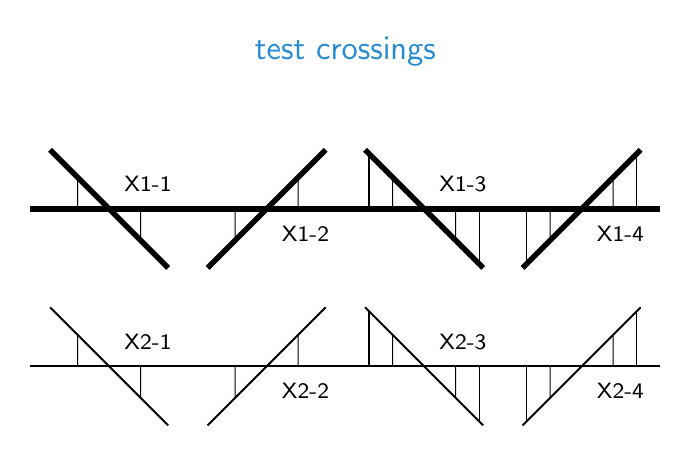
\begin{tikzpicture}[font=\sffamily]
    %!TEX TS-program = pdflatexmk
%!TEX root = test.tex

% Copyright (c) 2018 - 2021, Martin Scheidt (ISC license)
% Permission to use, copy, modify, and/or distribute this file for any purpose with or without fee is hereby granted, provided that the above copyright notice and this permission notice appear in all copies.

\node[blue] at (4,0) {\large test crossings};

\foreach \i in {1,2}{% base coordinate
  \coordinate (A\i) at ($(0,0) + 2*(0,-\i)$);% base coordinate
  \coordinate (B\i) at ($(8,0) + 2*(0,-\i)$);% base coordinate
}

\foreach \i in {1}{% draw main tracks on base coordinate
  \maintrack (A\i) --   (B\i);
}

\foreach \i in {2}{% draw secondary tracks on base coordinate
  \secondarytrack (A\i) --   (B\i);
}

\foreach \i in {1,2}{% coordinates for testing symbols
  \coordinate (X\i-1) at ($(1,0) + 2*(0,-\i)$);
  \coordinate (X\i-2) at ($(3,0) + 2*(0,-\i)$);
  \coordinate (X\i-3) at ($(5,0) + 2*(0,-\i)$);
  \coordinate (X\i-4) at ($(7,0) + 2*(0,-\i)$);
}

\foreach \i in {1}{% coordinates for testing symbols
  \maintrack (X\i-1) -- ++( 0.75,-0.75);
  \maintrack (X\i-1) -- ++(-0.75, 0.75);
  \maintrack (X\i-2) -- ++( 0.75, 0.75);
  \maintrack (X\i-2) -- ++(-0.75,-0.75);
  \maintrack (X\i-3) -- ++( 0.75,-0.75);
  \maintrack (X\i-3) -- ++(-0.75, 0.75);
  \maintrack (X\i-4) -- ++( 0.75, 0.75);
  \maintrack (X\i-4) -- ++(-0.75,-0.75);
}
\foreach \i in {2}{% coordinates for testing symbols
  \secondarytrack (X\i-1) -- ++( 0.75,-0.75);
  \secondarytrack (X\i-1) -- ++(-0.75, 0.75);
  \secondarytrack (X\i-2) -- ++( 0.75, 0.75);
  \secondarytrack (X\i-2) -- ++(-0.75,-0.75);
  \secondarytrack (X\i-3) -- ++( 0.75,-0.75);
  \secondarytrack (X\i-3) -- ++(-0.75, 0.75);
  \secondarytrack (X\i-4) -- ++( 0.75, 0.75);
  \secondarytrack (X\i-4) -- ++(-0.75,-0.75);
}

\crossing[branch=right]               at (X1-1) label (X1-1);
\crossing[branch=left ]               at (X1-2) label (X1-2);
\crossing[branch=right,fouling point] at (X1-3) label (X1-3);
\crossing[branch=left ,fouling point] at (X1-4) label (X1-4);

\crossing[branch=right]               at (X2-1) label (X2-1);
\crossing[branch=left ]               at (X2-2) label (X2-2);
\crossing[branch=right,fouling point] at (X2-3) label (X2-3);
\crossing[branch=left ,fouling point] at (X2-4) label (X2-4);

  \end{tikzpicture}

  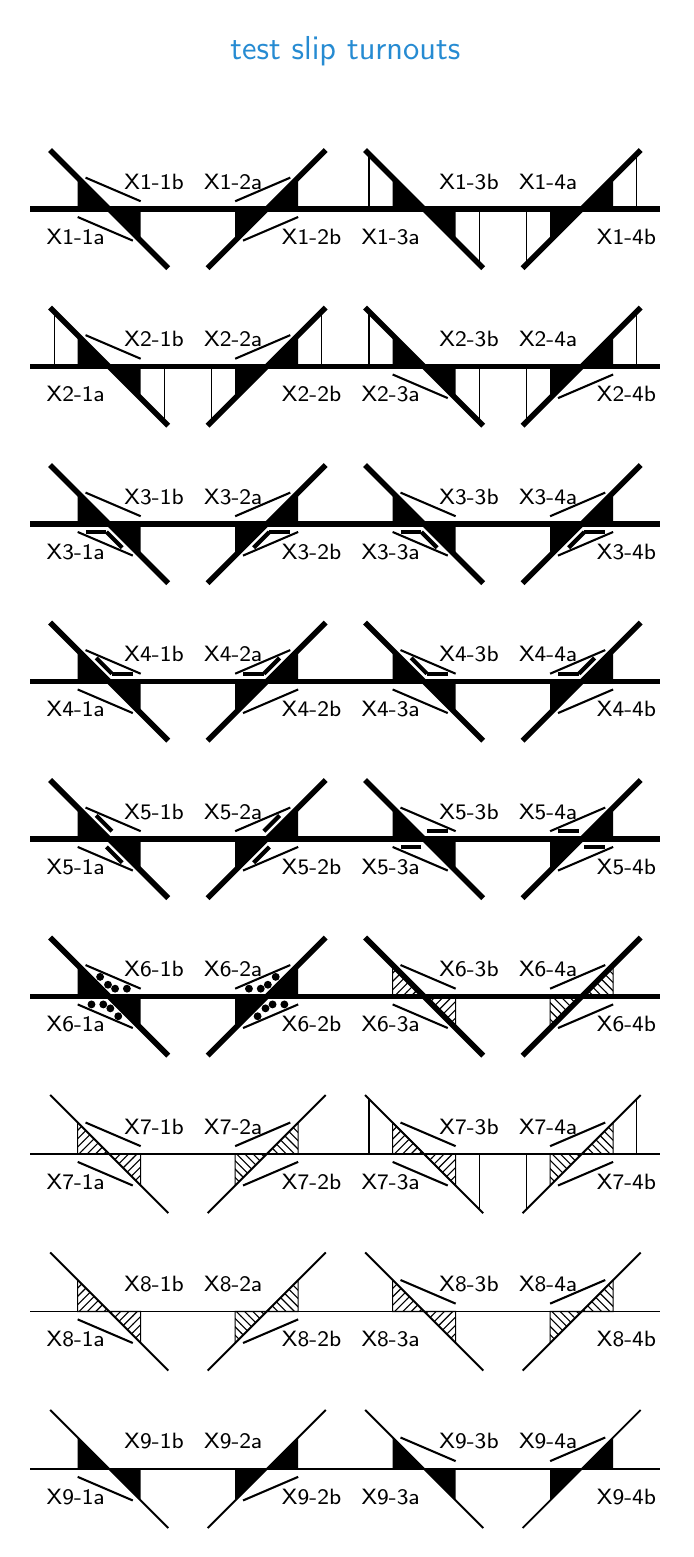
\begin{tikzpicture}[font=\sffamily]
    %!TEX TS-program = pdflatexmk
%!TEX root = test.tex

% Copyright (c) 2018 - 2022, Martin Scheidt (ISC license)
% Permission to use, copy, modify, and/or distribute this file for any purpose with or without fee is hereby granted, provided that the above copyright notice and this permission notice appear in all copies.

\node[blue] at (4,0) {\large test slip turnouts};

\foreach \i in {1,2,...,9}{% base coordinate
  \coordinate (A\i) at ($(0,0) + 2*(0,-\i)$);% base coordinate
  \coordinate (B\i) at ($(8,0) + 2*(0,-\i)$);% base coordinate
}

\foreach \i in {1,2,...,6}{% draw main tracks on base coordinate
  \maintrack (A\i) --   (B\i);
}

\foreach \i in {7,8,...,9}{% draw secondary tracks on base coordinate
  \secondarytrack (A\i) --   (B\i);
}

\foreach \i in {1,2,...,9}{% coordinates for testing symbols
  \coordinate (X\i-1) at ($(1,0) + 2*(0,-\i)$);
  \coordinate (X\i-2) at ($(3,0) + 2*(0,-\i)$);
  \coordinate (X\i-3) at ($(5,0) + 2*(0,-\i)$);
  \coordinate (X\i-4) at ($(7,0) + 2*(0,-\i)$);
}

\foreach \i in {1,2,...,6}{% coordinates for testing symbols
  \maintrack (X\i-1) -- ++( 0.75,-0.75);
  \maintrack (X\i-1) -- ++(-0.75, 0.75);
  \maintrack (X\i-2) -- ++( 0.75, 0.75);
  \maintrack (X\i-2) -- ++(-0.75,-0.75);
  \maintrack (X\i-3) -- ++( 0.75,-0.75);
  \maintrack (X\i-3) -- ++(-0.75, 0.75);
  \maintrack (X\i-4) -- ++( 0.75, 0.75);
  \maintrack (X\i-4) -- ++(-0.75,-0.75);
}

\foreach \i in {7,8,...,9}{% coordinates for testing symbols
  \secondarytrack (X\i-1) -- ++( 0.75,-0.75);
  \secondarytrack (X\i-1) -- ++(-0.75, 0.75);
  \secondarytrack (X\i-2) -- ++( 0.75, 0.75);
  \secondarytrack (X\i-2) -- ++(-0.75,-0.75);
  \secondarytrack (X\i-3) -- ++( 0.75,-0.75);
  \secondarytrack (X\i-3) -- ++(-0.75, 0.75);
  \secondarytrack (X\i-4) -- ++( 0.75, 0.75);
  \secondarytrack (X\i-4) -- ++(-0.75,-0.75);
}

\slipturnout[branch=right] at (X1-1) label (X1-1a)(X1-1b);
\slipturnout[branch=left ] at (X1-2) label (X1-2a)(X1-2b);
\slipturnout[branch=right,slip=none,fouling point] at (X1-3) label (X1-3a)(X1-3b);
\slipturnout[branch=left ,slip=none,fouling point] at (X1-4) label (X1-4a)(X1-4b);

\slipturnout[branch=right,slip=left ,fouling point] at (X2-1) label (X2-1a)(X2-1b);
\slipturnout[branch=left ,slip=left ,fouling point] at (X2-2) label (X2-2a)(X2-2b);
\slipturnout[branch=right,slip=right,fouling point] at (X2-3) label (X2-3a)(X2-3b);
\slipturnout[branch=left ,slip=right,fouling point] at (X2-4) label (X2-4a)(X2-4b);

\slipturnout[branch=right,forward points=right,backward points=left] at (X3-1) label (X3-1a)(X3-1b);
\slipturnout[branch=left ,forward points=right,backward points=left] at (X3-2) label (X3-2a)(X3-2b);
\slipturnout[branch=right,forward points=right,backward points=left] at (X3-3) label (X3-3a)(X3-3b);
\slipturnout[branch=left ,forward points=right,backward points=left] at (X3-4) label (X3-4a)(X3-4b);

\slipturnout[branch=right,forward points=left,backward points=right] at (X4-1) label (X4-1a)(X4-1b);
\slipturnout[branch=left ,forward points=left,backward points=right] at (X4-2) label (X4-2a)(X4-2b);
\slipturnout[branch=right,forward points=left,backward points=right] at (X4-3) label (X4-3a)(X4-3b);
\slipturnout[branch=left ,forward points=left,backward points=right] at (X4-4) label (X4-4a)(X4-4b);

\slipturnout[branch=right,forward points=right,backward points=right] at (X5-1) label (X5-1a)(X5-1b);
\slipturnout[branch=left ,forward points=left ,backward points=left] at (X5-2) label (X5-2a)(X5-2b);
\slipturnout[branch=right,forward points=left ,backward points=left ] at (X5-3) label (X5-3a)(X5-3b);
\slipturnout[branch=left ,forward points=right,backward points=right] at (X5-4) label (X5-4a)(X5-4b);

\slipturnout[branch=right,forward points=moving,backward points=moving] at (X6-1) label (X6-1a)(X6-1b);
\slipturnout[branch=left ,forward points=moving,backward points=moving] at (X6-2) label (X6-2a)(X6-2b);
\slipturnout[branch=right,operation=manual] at (X6-3) label (X6-3a)(X6-3b);
\slipturnout[branch=left ,operation=manual] at (X6-4) label (X6-4a)(X6-4b);

\slipturnout[branch=right,operation=manual] at (X7-1) label (X7-1a)(X7-1b);
\slipturnout[branch=left ,operation=manual] at (X7-2) label (X7-2a)(X7-2b);
\slipturnout[branch=right,operation=manual,fouling point] at (X7-3) label (X7-3a)(X7-3b);
\slipturnout[branch=left ,operation=manual,fouling point] at (X7-4) label (X7-4a)(X7-4b);

\slipturnout[branch=right,operation=manual,slip=right] at (X8-1) label (X8-1a)(X8-1b);
\slipturnout[branch=left ,operation=manual,slip=right] at (X8-2) label (X8-2a)(X8-2b);
\slipturnout[branch=right,operation=manual,slip=left ] at (X8-3) label (X8-3a)(X8-3b);
\slipturnout[branch=left ,operation=manual,slip=left ] at (X8-4) label (X8-4a)(X8-4b);

\slipturnout[branch=right,slip=right] at (X9-1) label (X9-1a)(X9-1b);
\slipturnout[branch=left ,slip=right] at (X9-2) label (X9-2a)(X9-2b);
\slipturnout[branch=right,slip=left ] at (X9-3) label (X9-3a)(X9-3b);
\slipturnout[branch=left ,slip=left ] at (X9-4) label (X9-4a)(X9-4b);

  \end{tikzpicture}

  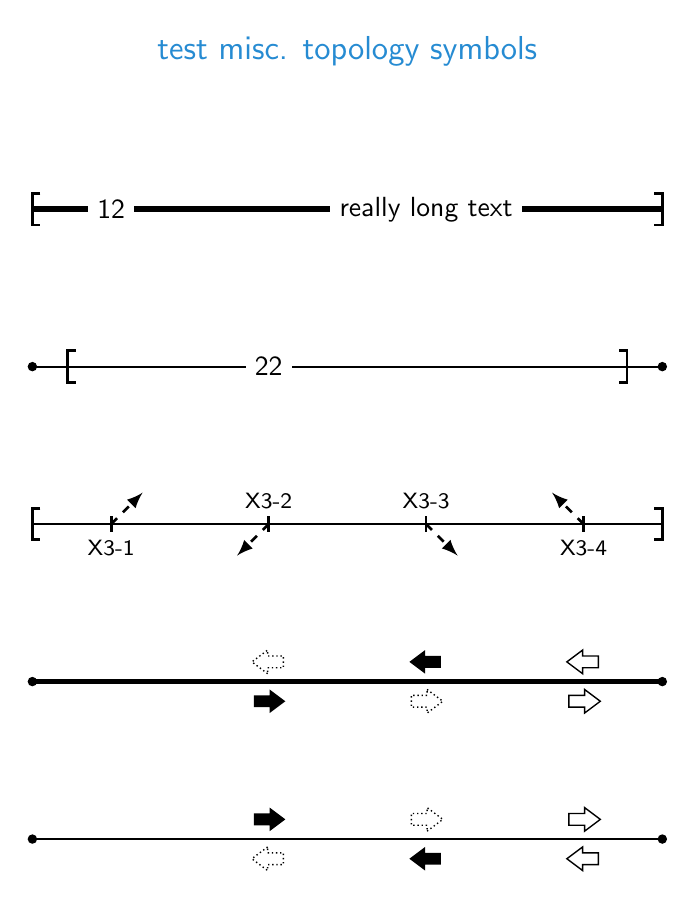
\begin{tikzpicture}[font=\sffamily]
    %!TEX TS-program = pdflatexmk
%!TEX root = test.tex

% Copyright (c) 2018 - 2021, Martin Scheidt (ISC license)
% Permission to use, copy, modify, and/or distribute this file for any purpose with or without fee is hereby granted, provided that the above copyright notice and this permission notice appear in all copies.

\node[blue] at (4,0) {\large test misc. topology symbols};

\foreach \i in {1,2,...,5}{% base coordinate
  \coordinate (A\i) at ($(0,0) + 2*(0,-\i)$);% base coordinate
  \coordinate (B\i) at ($(8,0) + 2*(0,-\i)$);% base coordinate
}

\foreach \i in {1,4}{% draw main tracks on base coordinate
  \maintrack (A\i) --   (B\i);
}

\foreach \i in {2,3,5}{% draw secondary tracks on base coordinate
  \secondarytrack (A\i) --   (B\i);
}

\foreach \i in {1,2,...,5}{% coordinates for testing symbols
  \coordinate (X\i-1) at ($(1,0) + 2*(0,-\i)$);
  \coordinate (X\i-2) at ($(3,0) + 2*(0,-\i)$);
  \coordinate (X\i-3) at ($(5,0) + 2*(0,-\i)$);
  \coordinate (X\i-4) at ($(7,0) + 2*(0,-\i)$);
}

\tracklabel at (X1-1) label (12);
\tracklabel at (X1-3) label (really long text);
\tracklabel at (X2-2) label (22);

\derailer[forward ,branch=left ] at (X3-1) label (X3-1);
\derailer[backward,branch=left ] at (X3-2) label (X3-2);
\derailer[forward ,branch=right] at (X3-3) label (X3-3);
\derailer[backward,branch=right] at (X3-4) label (X3-4);

\bufferstop[backward] at (A1);
\bufferstop[forward]  at (B1);
\bufferstop[backward,friction=.5]  at (A2);
\bufferstop[forward ,friction=.5]  at (B2);
\bufferstop[backward] at (A3);
\bufferstop[forward]  at (B3);

\trackclosure at (A4);
\directioncontrol[forward] at (X4-2);
\directioncontrol[backward] at (X4-3);
\directioncontrol[bidirectional] at (X4-4);
\trackclosure at (B4);

\trackclosure at (A5);
\directioncontrol[forward,position=left] at (X5-2);
\directioncontrol[backward,position=left] at (X5-3);
\directioncontrol[bidirectional,position=left] at (X5-4);
\trackclosure at (B5);

  \end{tikzpicture}

  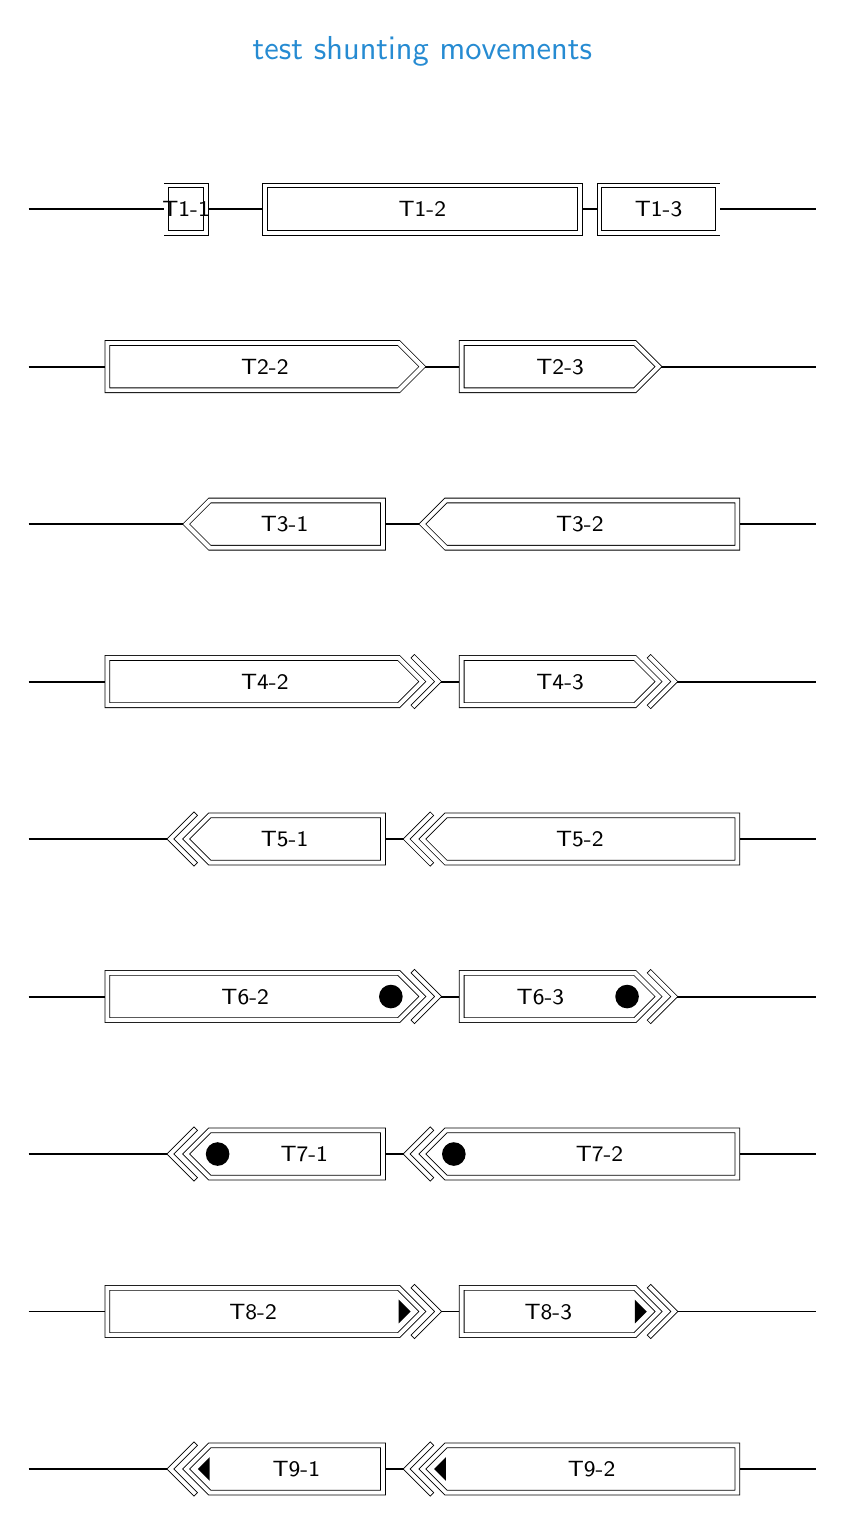
\begin{tikzpicture}[font=\sffamily]
    %!TEX TS-program = pdflatexmk
%!TEX root = test.tex

% Copyright (c) 2018 - 2022, Martin Scheidt (ISC license)
% Permission to use, copy, modify, and/or distribute this file for any purpose with or without fee is hereby granted, provided that the above copyright notice and this permission notice appear in all copies.

\node[blue] at (4,0) {\large test shunting movements};

\foreach \i in {1,2,...,9}{% base coordinate
  \coordinate (A\i) at ($(-1,0) + 2*(0,-\i)$);
  \coordinate (B\i) at ($( 9,0) + 2*(0,-\i)$);
}

\foreach \i in {1,2,...,9}{% draw main tracks on base coordinate
  \secondarytrack (A\i) --   (B\i);
}

\foreach \i in {1,2,...,9}{% coordinates for testing symbols
  \coordinate (T\i-1) at ($(1,0) + 2*(0,-\i)$);
  \coordinate (T\i-2) at ($(4,0) + 2*(0,-\i)$);
  \coordinate (T\i-3) at ($(7,0) + 2*(0,-\i)$);
}

\parkedvehicles[length=0.5cm] at (T1-1) label (T1-1);
\parkedvehicles[]             at (T1-2) label (T1-2);
\parkedvehicles[length=1.5cm] at (T1-3) label (T1-3);

\shunting[forward]               at (T2-2) label (T2-2);
\shunting[forward ,length=2.5cm] at (T2-3) label (T2-3);
\shunting[backward,length=2.5cm] at (T3-1) label (T3-1);
\shunting[backward]              at (T3-2) label (T3-2);

\shunting[movement,forward]               at (T4-2) label (T4-2);
\shunting[movement,forward ,length=2.5cm] at (T4-3) label (T4-3);
\shunting[movement,backward,length=2.5cm] at (T5-1) label (T5-1);
\shunting[movement,backward]              at (T5-2) label (T5-2);

\shunting[operation=manual,movement,forward]               at (T6-2) label (T6-2);
\shunting[operation=manual,movement,forward ,length=2.5cm] at (T6-3) label (T6-3);
\shunting[operation=manual,movement,backward,length=2.5cm] at (T7-1) label (T7-1);
\shunting[operation=manual,movement,backward]              at (T7-2) label (T7-2);

\shunting[operation=automatic,movement,forward]               at (T8-2) label (T8-2);
\shunting[operation=automatic,movement,forward ,length=2.5cm] at (T8-3) label (T8-3);
\shunting[operation=automatic,movement,backward,length=2.5cm] at (T9-1) label (T9-1);
\shunting[operation=automatic,movement,backward]              at (T9-2) label (T9-2);

  \end{tikzpicture}

  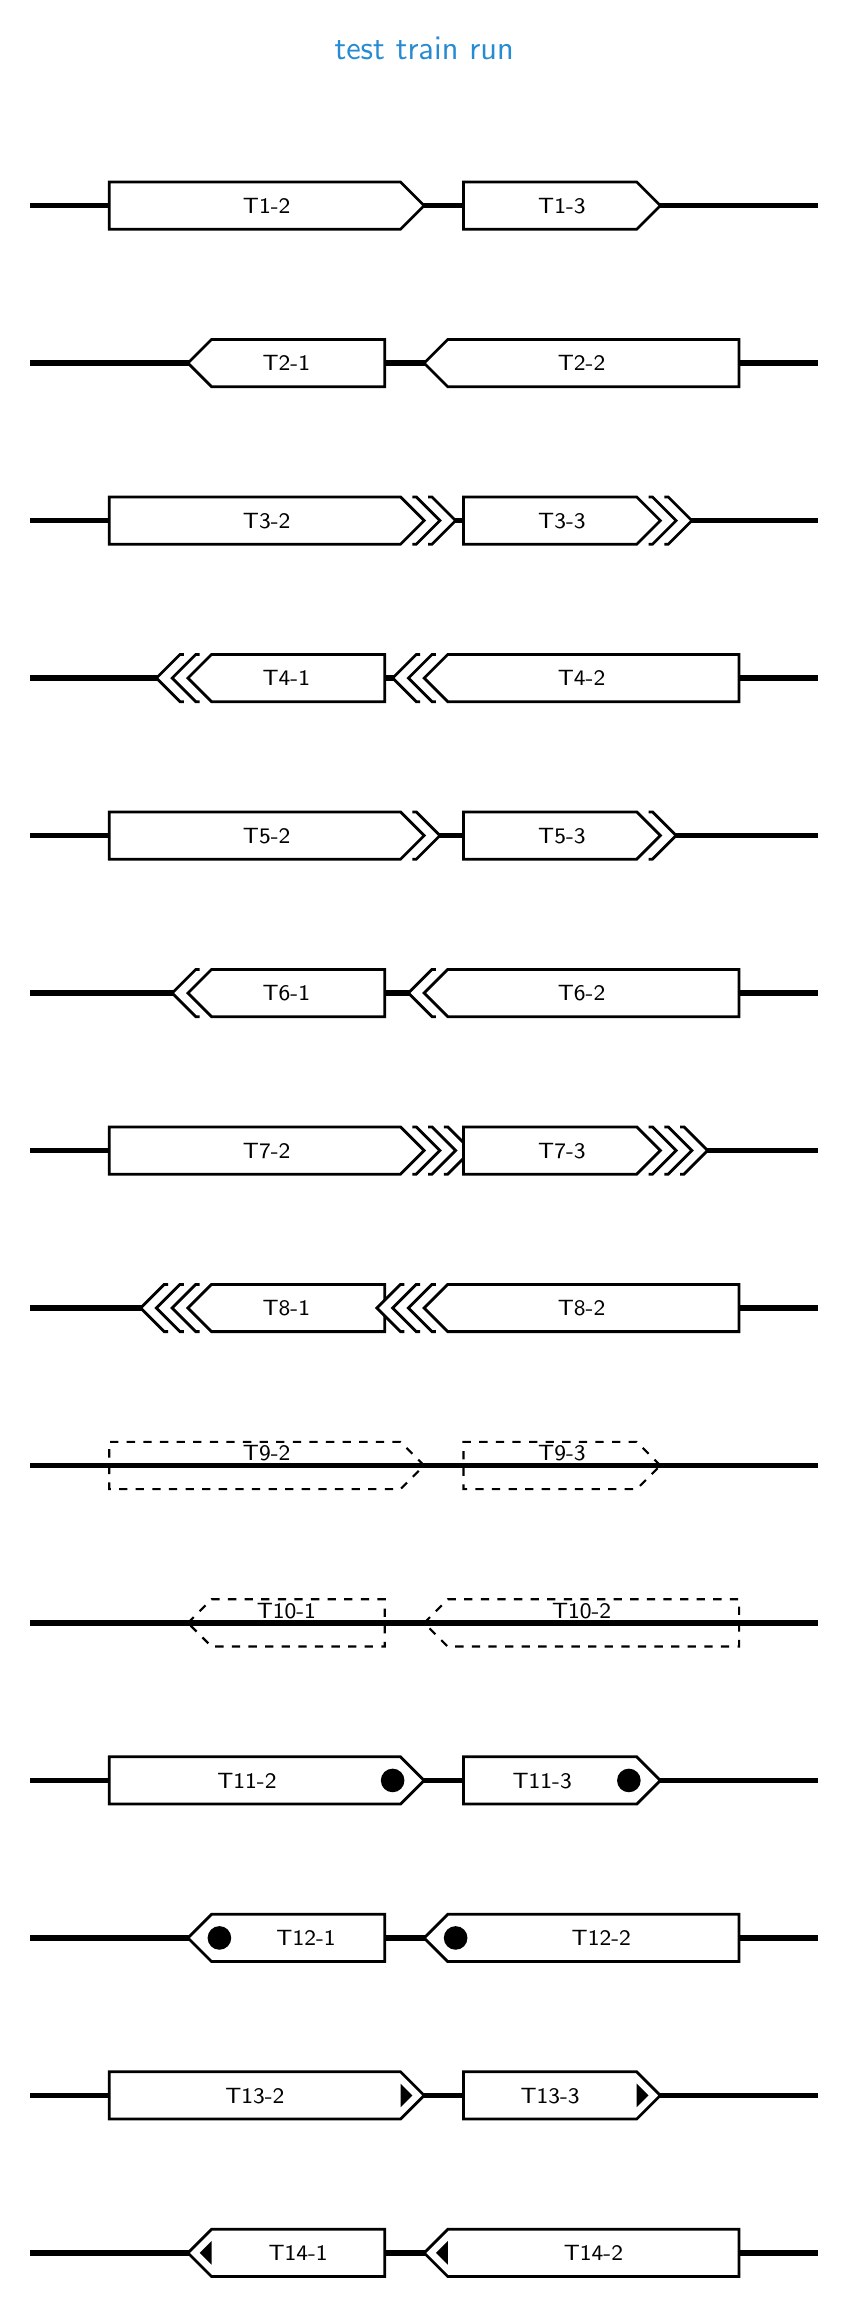
\begin{tikzpicture}[font=\sffamily]
    %!TEX TS-program = pdflatexmk
%!TEX root = test.tex

% Copyright (c) 2018 - 2021, Martin Scheidt (ISC license)
% Permission to use, copy, modify, and/or distribute this file for any purpose with or without fee is hereby granted, provided that the above copyright notice and this permission notice appear in all copies.

\node[blue] at (4,0) {\large test train run};

\foreach \i in {1,2,...,14}{% base coordinate
  \coordinate (A\i) at ($(-1,0) + 2*(0,-\i)$);
  \coordinate (B\i) at ($( 9,0) + 2*(0,-\i)$);
}

\foreach \i in {1,2,...,14}{% draw main tracks on base coordinate
  \maintrack (A\i) --   (B\i);
}

\foreach \i in {1,2,...,14}{% coordinates for testing symbols
  \coordinate (T\i-1) at ($(1,0) + 2*(0,-\i)$);
  \coordinate (T\i-2) at ($(4,0) + 2*(0,-\i)$);
  \coordinate (T\i-3) at ($(7,0) + 2*(0,-\i)$);
}

\train[forward]               at (T1-2) label (T1-2);
\train[forward ,length=2.5cm] at (T1-3) label (T1-3);
\train[backward,length=2.5cm] at (T2-1) label (T2-1);
\train[backward]              at (T2-2) label (T2-2);

\train[run=normal,forward]               at (T3-2) label (T3-2);
\train[run=normal,forward ,length=2.5cm] at (T3-3) label (T3-3);
\train[run=normal,backward,length=2.5cm] at (T4-1) label (T4-1);
\train[run=normal,backward]              at (T4-2) label (T4-2);

\train[run=slow,forward]               at (T5-2) label (T5-2);
\train[run=slow,forward ,length=2.5cm] at (T5-3) label (T5-3);
\train[run=slow,backward,length=2.5cm] at (T6-1) label (T6-1);
\train[run=slow,backward]              at (T6-2) label (T6-2);

\train[run=fast,forward]               at (T7-2) label (T7-2);
\train[run=fast,forward ,length=2.5cm] at (T7-3) label (T7-3);
\train[run=fast,backward,length=2.5cm] at (T8-1) label (T8-1);
\train[run=fast,backward]              at (T8-2) label (T8-2);

\train[ghost,forward]               at (T9-2) label (T9-2);
\train[ghost,forward ,length=2.5cm] at (T9-3) label (T9-3);
\train[ghost,backward,length=2.5cm] at (T10-1) label (T10-1);
\train[ghost,backward]              at (T10-2) label (T10-2);

\train[operation=manual,forward]               at (T11-2) label (T11-2);
\train[operation=manual,forward ,length=2.5cm] at (T11-3) label (T11-3);
\train[operation=manual,backward,length=2.5cm] at (T12-1) label (T12-1);
\train[operation=manual,backward]              at (T12-2) label (T12-2);

\train[operation=automatic,forward]               at (T13-2) label (T13-2);
\train[operation=automatic,forward ,length=2.5cm] at (T13-3) label (T13-3);
\train[operation=automatic,backward,length=2.5cm] at (T14-1) label (T14-1);
\train[operation=automatic,backward]              at (T14-2) label (T14-2);

  \end{tikzpicture}

  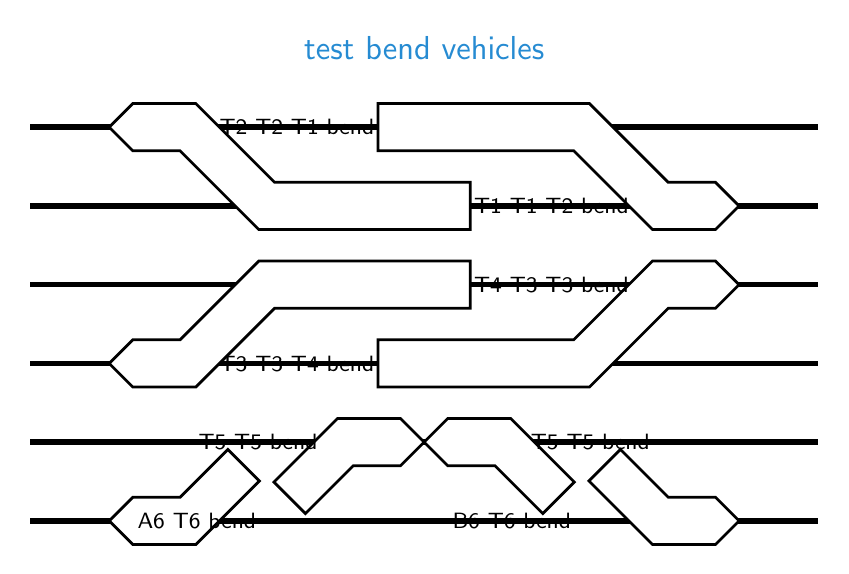
\begin{tikzpicture}[font=\sffamily]
    %!TEX TS-program = pdflatexmk
%!TEX root = test.tex

% Copyright (c) 2018 - 2022, Martin Scheidt (ISC license)
% Permission to use, copy, modify, and/or distribute this file for any purpose with or without fee is hereby granted, provided that the above copyright notice and this permission notice appear in all copies.

\node[blue] at (4,0) {\large test bend vehicles};

\foreach \i in {1,2,...,6}{% base coordinate
  \coordinate (A\i) at ($(-1,0) + (0,-\i)$);
  \coordinate (B\i) at ($( 9,0) + (0,-\i)$);
}

\foreach \i in {1,2,...,6}{% draw main tracks on base coordinate
  \maintrack (A\i) --   (B\i);
}

\foreach \i in {1,2,...,6}{% coordinates for testing symbols
  \coordinate (T\i-0) at ($(0,0) + (0,-\i)$);
  \coordinate (T\i-1) at ($(1,0) + (0,-\i)$);
  \coordinate (T\i-2) at ($(2,0) + (0,-\i)$);
  \coordinate (T\i-3) at ($(3,0) + (0,-\i)$);
  \coordinate (T\i-4) at ($(4,0) + (0,-\i)$);
  \coordinate (T\i-5) at ($(5,0) + (0,-\i)$);
  \coordinate (T\i-6) at ($(6,0) + (0,-\i)$);
  \coordinate (T\i-7) at ($(7,0) + (0,-\i)$);
  \coordinate (T\i-8) at ($(8,0) + (0,-\i)$);
}

\train[forward, length=5cm,
  bend right at={(T1-6)}, bend left at={(T2-7)},
  shift label={(T1-6)}, label align=left] at (T2-8) label (T2 T2 T1 bend);
\train[forward, length=5cm,
  bend left at={(T4-6)},bend right at={(T3-7)},
  shift label={(T4-6)}, label align=left] at (T3-8) label (T3 T3 T4 bend);
\train[backward, length=5cm,
  bend right at={(T1-1)}, bend left at={(T2-2)},
  shift label={(T2-2)}, label align=right] at (T1-0) label (T1 T1 T2 bend);
\train[backward, length=5cm,
  bend left at={(T4-1)},bend right at={(T3-2)},
  shift label={(T3-2)}, label align=right] at (T4-0) label (T4 T3 T3 bend);
\train[backward, length=2cm,
  bend left at={(T6-1)},
  shift label={(T6-1)}, label align=left] at (T6-0) label (A6 T6 bend);
\train[forward, length=2cm,
  bend right at={(T5-3)},
  shift label={(T5-2)}, label align=right] at (T5-4) label (T5 T5 bend);
\train[backward, length=2cm,
  bend right at={(T5-5)},
  shift label={(T5-6)}, label align=left] at (T5-4) label (T5 T5 bend);
\train[forward, length=2cm,
  bend left at={(T6-7)},
  shift label={(T6-7)}, label align=left] at (T6-8) label (B6 T6 bend);

  \end{tikzpicture}

  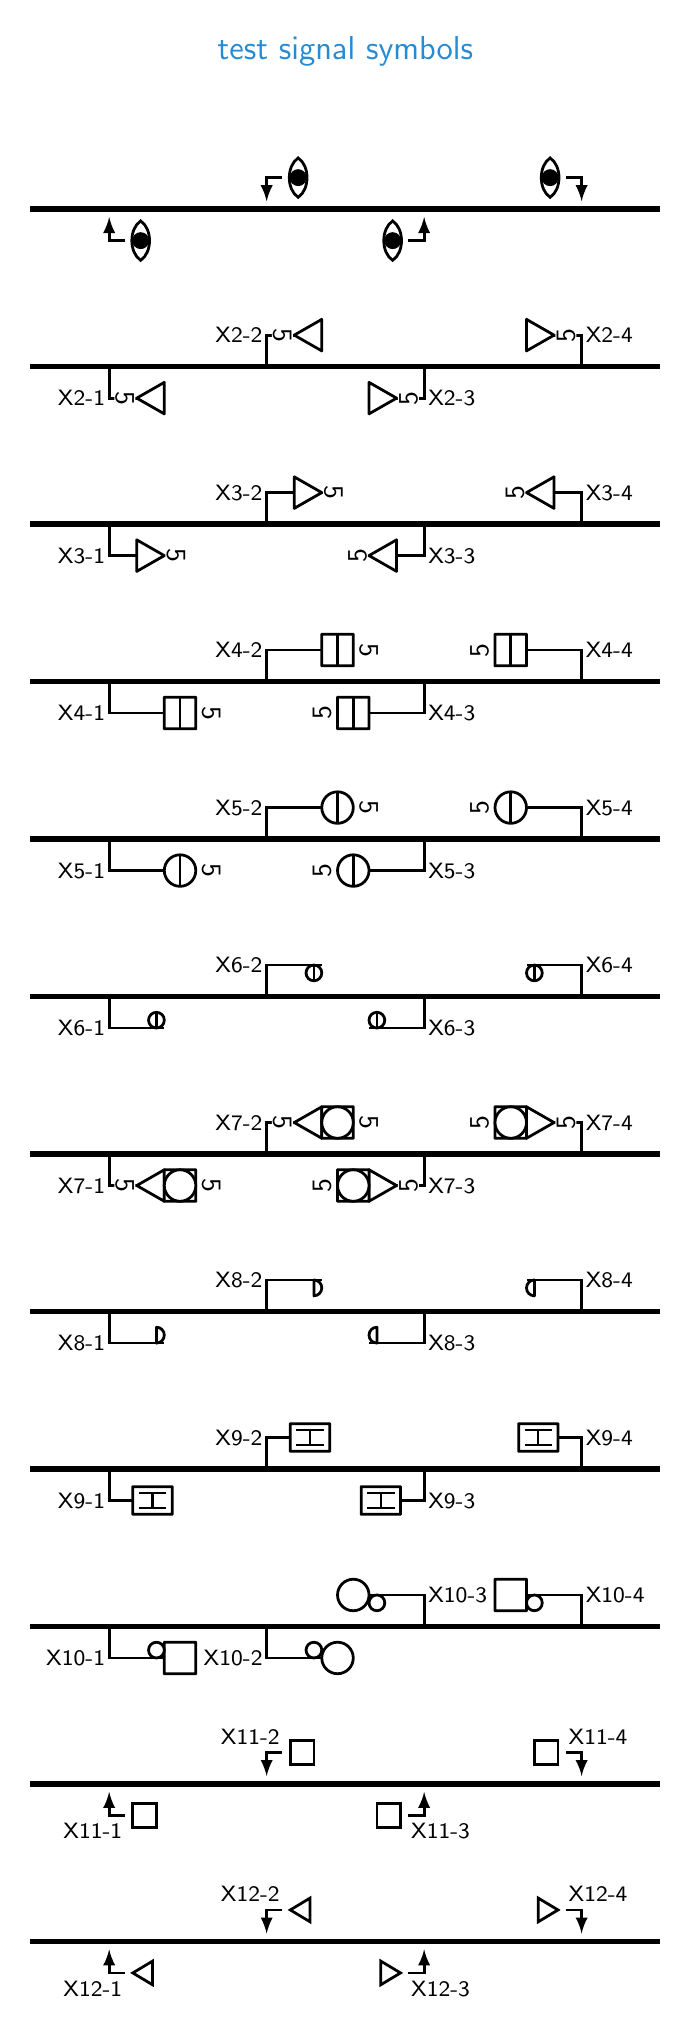
\begin{tikzpicture}[font=\sffamily]
    %!TEX TS-program = pdflatexmk
%!TEX root = test.tex

% Copyright (c) 2018 - 2020, Martin Scheidt (ISC license)
% Permission to use, copy, modify, and/or distribute this file for any purpose with or without fee is hereby granted, provided that the above copyright notice and this permission notice appear in all copies.

\node[blue] at (4,0) {\large test signal symbols};

\foreach \i in {1,2,...,12}{% base coordinate
  \coordinate (A\i) at ($(0,0) + 2*(0,-\i)$);% base coordinate
  \coordinate (B\i) at ($(8,0) + 2*(0,-\i)$);% base coordinate
}

\foreach \i in {1,2,...,12}{% draw main tracks on base coordinate
  \maintrack (A\i) --   (B\i);
}

\foreach \i in {1,2,...,12}{% coordinates for testing symbols
  \coordinate (X\i-1) at ($(1,0) + 2*(0,-\i)$);
  \coordinate (X\i-2) at ($(3,0) + 2*(0,-\i)$);
  \coordinate (X\i-3) at ($(5,0) + 2*(0,-\i)$);
  \coordinate (X\i-4) at ($(7,0) + 2*(0,-\i)$);
}

\viewpoint[forward ] at (X1-1);
\viewpoint[forward ,position=left] at (X1-2);
\viewpoint[backward,position=left] at (X1-3);
\viewpoint[backward] at (X1-4);

\distantsignal[forward ,distant speed=5] at (X2-1) label (X2-1);
\distantsignal[forward ,distant speed=5,position=left] at (X2-2) label (X2-2);
\distantsignal[backward,distant speed=5,position=left] at (X2-3) label (X2-3);
\distantsignal[backward,distant speed=5] at (X2-4) label (X2-4);

\speedsignal[forward ,speed=5] at (X3-1) label (X3-1);
\speedsignal[forward ,speed=5,position=left] at (X3-2) label (X3-2);
\speedsignal[backward,speed=5,position=left] at (X3-3) label (X3-3);
\speedsignal[backward,speed=5] at (X3-4) label (X3-4);

\blocksignal[forward ,locked,speed=5] at (X4-1) label (X4-1);
\blocksignal[forward ,locked,speed=5,position=left] at (X4-2) label (X4-2);
\blocksignal[backward,locked,speed=5,position=left] at (X4-3) label (X4-3);
\blocksignal[backward,locked,speed=5] at (X4-4) label (X4-4);

\routesignal[forward ,locked,speed=5] at (X5-1) label (X5-1);
\routesignal[forward ,locked,speed=5,position=left] at (X5-2) label (X5-2);
\routesignal[backward,locked,speed=5,position=left] at (X5-3) label (X5-3);
\routesignal[backward,locked,speed=5] at (X5-4) label (X5-4);

\shuntsignal[forward ,locked] at (X6-1) label (X6-1);
\shuntsignal[forward ,locked,position=left] at (X6-2) label (X6-2);
\shuntsignal[backward,locked,position=left] at (X6-3) label (X6-3);
\shuntsignal[backward,locked] at (X6-4) label (X6-4);

\signal[forward ,distant,block,route,distant speed=5,speed=5] at (X7-1) label (X7-1);
\signal[forward ,distant,block,route,distant speed=5,speed=5,position=left] at (X7-2) label (X7-2);
\signal[backward,distant,block,route,distant speed=5,speed=5,position=left] at (X7-3) label (X7-3);
\signal[backward,distant,block,route,distant speed=5,speed=5] at (X7-4) label (X7-4);

\shuntlimit[forward ] at (X8-1) label (X8-1);
\shuntlimit[forward ,position=left] at (X8-2) label (X8-2);
\shuntlimit[backward,position=left] at (X8-3) label (X8-3);
\shuntlimit[backward] at (X8-4) label (X8-4);

\berthsignal[forward ] at (X9-1) label (X9-1);
\berthsignal[forward ,position=left] at (X9-2) label (X9-2);
\berthsignal[backward,position=left] at (X9-3) label (X9-3);
\berthsignal[backward] at (X9-4) label (X9-4);

\signal[forward ,block,shunting] at (X10-1) label (X10-1);
\signal[forward ,route,shunting] at (X10-2) label (X10-2);
\signal[backward,route,shunting] at (X10-3) label (X10-3);
\signal[backward,block,shunting] at (X10-4) label (X10-4);

\movementauthority[forward ] at (X11-1) label (X11-1);
\movementauthority[forward ,position=left] at (X11-2) label (X11-2);
\movementauthority[backward,position=left] at (X11-3) label (X11-3);
\movementauthority[backward] at (X11-4) label (X11-4);

\brakingpoint[forward ] at (X12-1) label (X12-1);
\brakingpoint[forward ,position=left] at (X12-2) label (X12-2);
\brakingpoint[backward,position=left] at (X12-3) label (X12-3);
\brakingpoint[backward] at (X12-4) label (X12-4);

  \end{tikzpicture}

  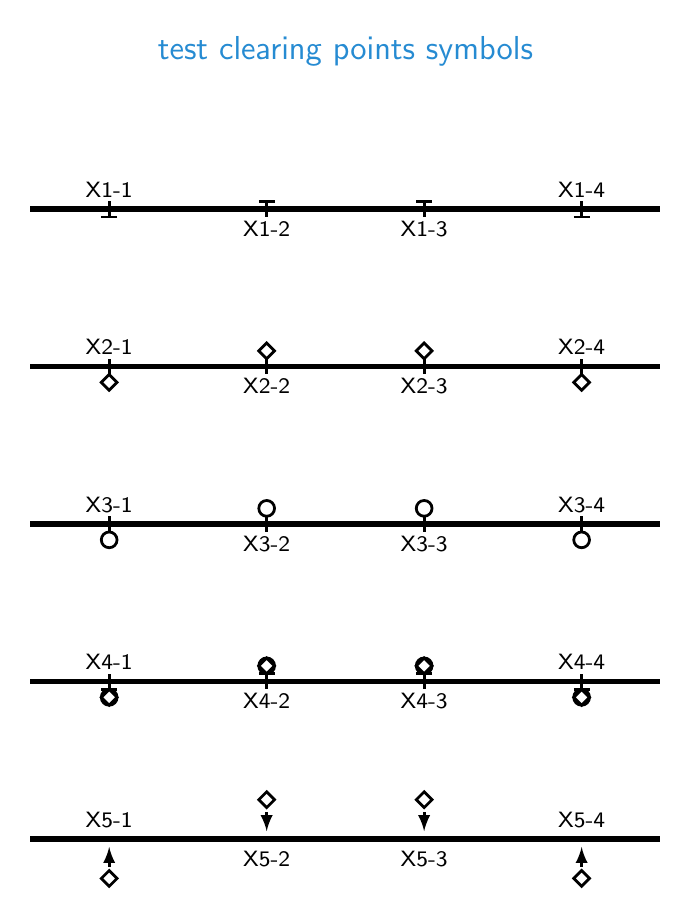
\begin{tikzpicture}[font=\sffamily]
    %!TEX TS-program = pdflatexmk
%!TEX root = test.tex

% Copyright (c) 2018 - 2020, Martin Scheidt (ISC license)
% Permission to use, copy, modify, and/or distribute this file for any purpose with or without fee is hereby granted, provided that the above copyright notice and this permission notice appear in all copies.

\node[blue] at (4,0) {\large test clearing points symbols};

\foreach \i in {1,2,...,5}{% base coordinate
  \coordinate (A\i) at ($(0,0) + 2*(0,-\i)$);% base coordinate
  \coordinate (B\i) at ($(8,0) + 2*(0,-\i)$);% base coordinate
}

\foreach \i in {1,2,...,5}{% draw main tracks on base coordinate
  \maintrack (A\i) --   (B\i);
}

\foreach \i in {1,2,...,5}{% coordinates for testing symbols
  \coordinate (X\i-1) at ($(1,0) + 2*(0,-\i)$);
  \coordinate (X\i-2) at ($(3,0) + 2*(0,-\i)$);
  \coordinate (X\i-3) at ($(5,0) + 2*(0,-\i)$);
  \coordinate (X\i-4) at ($(7,0) + 2*(0,-\i)$);
}

\clearingpoint[] at (X1-1) label (X1-1);
\clearingpoint[backward] at (X1-2) label (X1-2);
\clearingpoint[forward ,position=left] at (X1-3) label (X1-3);
\clearingpoint[backward,position=left] at (X1-4) label (X1-4);

\blockclearing[] at (X2-1) label (X2-1);
\blockclearing[backward] at (X2-2) label (X2-2);
\blockclearing[forward ,position=left] at (X2-3) label (X2-3);
\blockclearing[backward,position=left] at (X2-4) label (X2-4);

\routeclearing[] at (X3-1) label (X3-1);
\routeclearing[backward] at (X3-2) label (X3-2);
\routeclearing[forward ,position=left] at (X3-3) label (X3-3);
\routeclearing[backward,position=left] at (X3-4) label (X3-4);

\clearingpoint[standard,route,block,forward ] at (X4-1) label (X4-1);
\clearingpoint[standard,route,block,backward] at (X4-2) label (X4-2);
\clearingpoint[standard,route,block,forward ,position=left] at (X4-3) label (X4-3);
\clearingpoint[standard,route,block,backward,position=left] at (X4-4) label (X4-4);

\dangerpoint[forward] at (X5-1) label (X5-1);
\dangerpoint[backward] at (X5-2) label (X5-2);
\dangerpoint[forward ,position=left] at (X5-3) label (X5-3);
\dangerpoint[backward,position=left] at (X5-4) label (X5-4);
  \end{tikzpicture}

  \begin{tikzpicture}[font=\sffamily]
    %!TEX TS-program = pdflatexmk
%!TEX root = ../snippets.tex

% Copyright (c) 2018 - 2021, Martin Scheidt (ISC license)
% Permission to use, copy, modify, and/or distribute this file for any purpose with or without fee is hereby granted, provided that the above copyright notice and this permission notice appear in all copies.

\coordinate (A)  at (0,0);
\coordinate (B)  at (6,0);
\coordinate (T1) at (2,0);
\coordinate (T2) at (4,0);

\maintrack (A) -- (B);

\balise[]              at (T1) label ();
\balise[position=left] at (T2) label ();
  \end{tikzpicture}

  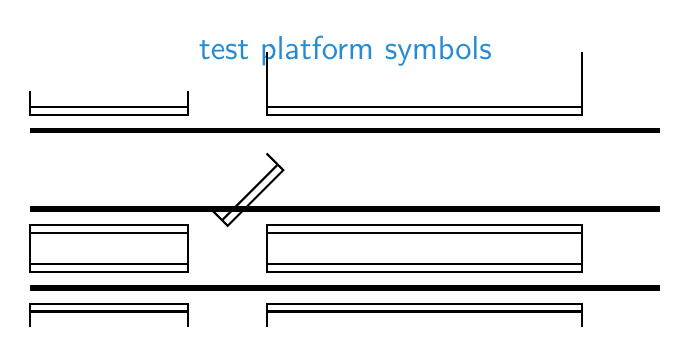
\begin{tikzpicture}[font=\sffamily]
    %!TEX TS-program = pdflatexmk
%!TEX root = test.tex

% Copyright (c) 2018 - 2022, Martin Scheidt (ISC license)
% Permission to use, copy, modify, and/or distribute this file for any purpose with or without fee is hereby granted, provided that the above copyright notice and this permission notice appear in all copies.

\node[blue] at (4,0) {\large test platform symbols};

\foreach \i in {1,2,...,3}{% base coordinate
  \coordinate (A\i) at ($(0,0) + (0,-\i)$);% base coordinate
  \coordinate (B\i) at ($(8,0) + (0,-\i)$);% base coordinate
}

\foreach \i in {1,2,...,3}{% draw main tracks on base coordinate
  \maintrack (A\i) --   (B\i);
}

\foreach \i in {1,2,...,3}{% coordinates for testing symbols
  \coordinate (X\i-1) at ($(1,0) + (0,-\i)$);
  \coordinate (X\i-2) at ($(3,0) + (0,-\i)$);
  \coordinate (X\i-3) at ($(5,0) + (0,-\i)$);
  \coordinate (X\i-4) at ($(7,0) + (0,-\i)$);
}

\platform[side=left,length=2cm] at (X1-1);
\platform[side=left,width=1cm]  at (X1-3);

\platform[side=left,length=1cm,rotate=45] at (X2-2);

\platform[side=right,length=2cm] at (X2-1);
\platform[side=right] at (X2-3);

\platform[side=both,length=2cm] at (X3-1);
\platform[side=both] at (X3-3);

  \end{tikzpicture}

  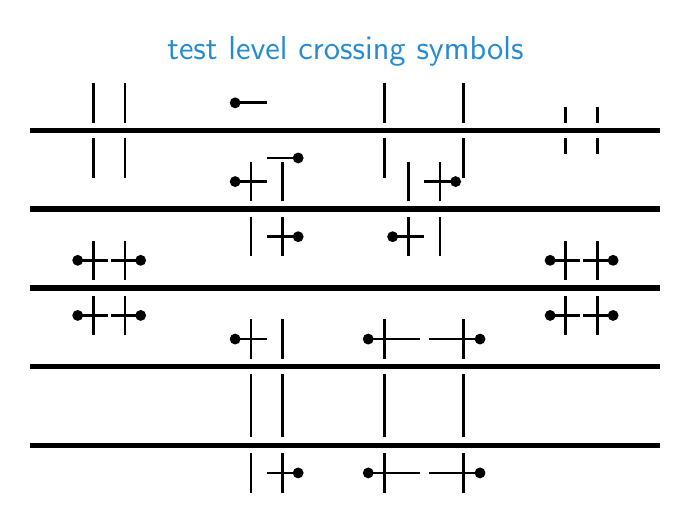
\begin{tikzpicture}[font=\sffamily]
    %!TEX TS-program = pdflatexmk
%!TEX root = test.tex

% Copyright (c) 2018 - 2022, Martin Scheidt (ISC license)
% Permission to use, copy, modify, and/or distribute this file for any purpose with or without fee is hereby granted, provided that the above copyright notice and this permission notice appear in all copies.

\node[blue] at (4,0) {\large test level crossing symbols};

\foreach \i in {1,2,...,5}{% base coordinate
  \coordinate (A\i) at ($(0,0) + (0,-\i)$);% base coordinate
  \coordinate (B\i) at ($(8,0) + (0,-\i)$);% base coordinate
}

\foreach \i in {1,2,...,5}{% draw main tracks on base coordinate
  \maintrack (A\i) --   (B\i);
}

\foreach \i in {1,2,...,5}{% coordinates for testing symbols
  \coordinate (X\i-1) at ($(1,0) + (0,-\i)$);
  \coordinate (X\i-2) at ($(3,0) + (0,-\i)$);
  \coordinate (X\i-3) at ($(5,0) + (0,-\i)$);
  \coordinate (X\i-4) at ($(7,0) + (0,-\i)$);
}

\levelcrossing[] at (X1-1);
\levelcrossing[no road,barrier=semi] at (X1-2);
\levelcrossing[road width=1cm] at (X1-3);
\levelcrossing[width=0.2cm] at (X1-4);

\levelcrossing[barrier=semi] at (X2-2);
\levelcrossing[barrier=semi,position=left] at (X2-3);

\levelcrossing[barrier=full] at (X3-1);
\levelcrossing[barrier=full,position=left] at (X3-4);

\levelcrossing[barrier=semi,side=left]  at (X4-2);
\levelcrossing[barrier=semi,side=right] at (X5-2);

\levelcrossing[road width=1cm,barrier=full,side=left]  at (X4-3);
\levelcrossing[road width=1cm,barrier=full,side=right] at (X5-3);
  \end{tikzpicture}

  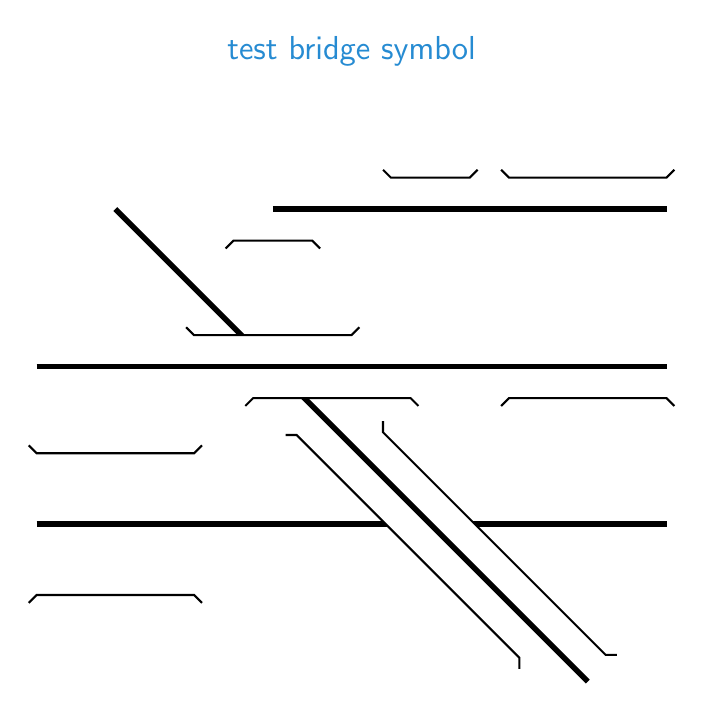
\begin{tikzpicture}[font=\sffamily]
    %!TEX TS-program = pdflatexmk
%!TEX root = test.tex

% Copyright (c) 2018 - 2022, Martin Scheidt (ISC license)
% Permission to use, copy, modify, and/or distribute this file for any purpose with or without fee is hereby granted, provided that the above copyright notice and this permission notice appear in all copies.

\node[blue] at (4,0) {\large test bridge symbol};

\foreach \i in {1,2,...,4}{% base coordinate
  \coordinate (A\i) at ($(0,0) + 2*(0,-\i)$);% base coordinate
  \coordinate (B\i) at ($(8,0) + 2*(0,-\i)$);% base coordinate
}


\foreach \i in {1,2,...,4}{% coordinates for testing symbols
  \coordinate (X\i-1) at ($(1,0) + 2*(0,-\i)$);
  \coordinate (X\i-2) at ($(3,0) + 2*(0,-\i)$);
  \coordinate (X\i-3) at ($(5,0) + 2*(0,-\i)$);
  \coordinate (X\i-4) at ($(7,0) + 2*(0,-\i)$);
}

\bridge[length=2cm,width=1cm] at (X3-1);
\maintrack (A3) -- (B3);
\bridge[rotate=-45,shift left=0.75cm] at (X3-3);
\maintrack (X1-1) -- (X4-4);
\bridge[length=2cm,shift right=0.75cm] at (X2-2);
\bridge[length=2cm,width=1.5cm] at (7,-3);
\maintrack (A2) -- (B2);
\maintrack (X1-2) -- (B1);

\bridge[no background,length=1cm,side=right] at (X1-2);
\bridge[no background,length=1cm,side=left]  at (X1-3);
  \end{tikzpicture}

  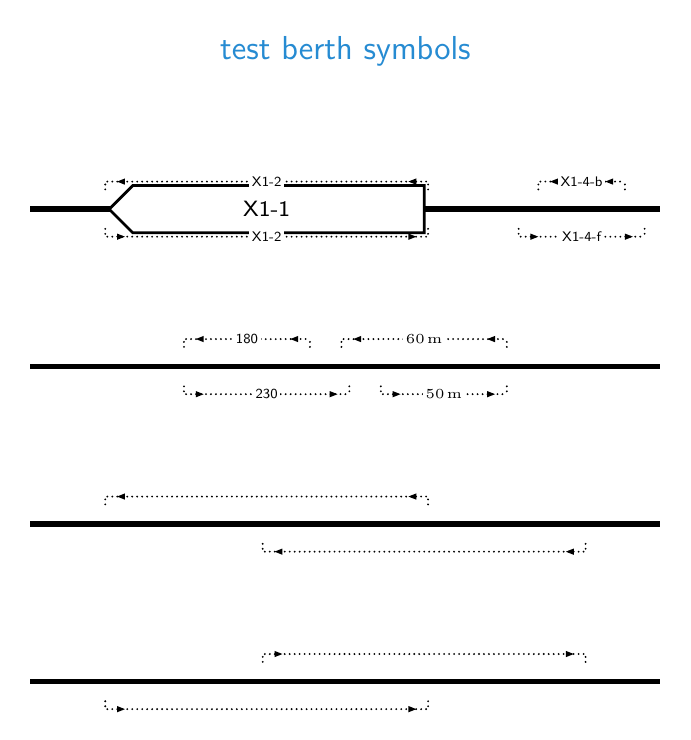
\begin{tikzpicture}[font=\sffamily]
    %!TEX TS-program = pdflatexmk
%!TEX root = test.tex

% Copyright (c) 2018 - 2022, Martin Scheidt (ISC license)
% Permission to use, copy, modify, and/or distribute this file for any purpose with or without fee is hereby granted, provided that the above copyright notice and this permission notice appear in all copies.

\node[blue] at (4,0) {\large test berth symbols};

\foreach \i in {1,2,...,4}{% base coordinate
  \coordinate (A\i) at ($(0,0) + 2*(0,-\i)$);% base coordinate
  \coordinate (B\i) at ($(8,0) + 2*(0,-\i)$);% base coordinate
}

\foreach \i in {1,2,...,4}{% draw main tracks on base coordinate
  \maintrack (A\i) --   (B\i);
}

\foreach \i in {1,2,...,4}{% coordinates for testing symbols
  \coordinate (X\i-1) at ($(1,0) + 2*(0,-\i)$);
  \coordinate (X\i-2) at ($(3,0) + 2*(0,-\i)$);
  \coordinate (X\i-3) at ($(5,0) + 2*(0,-\i)$);
  \coordinate (X\i-4) at ($(7,0) + 2*(0,-\i)$);
}

\train[backward] at (X1-1) label (X1-1);

\berth[bidirectional]  at (X1-2) length (X1-2);
\berth[forward,length=1.5cm] at (X1-4) length (X1-4-f);
\berth[backward,length=1cm]  at (X1-4) length (X1-4-b);

\berth[forward,length=2cm]    at                   (X2-2) length (230);
\berth[backward,length=1.5cm] at ([shift={(-0.25,0)}] X2-2) length (180);
\berth[forward,length=1.5cm]  at ([shift={( 0.25,0)}] X2-3) length (\SI{50}{\metre});
\berth[backward,length=2cm]   at                   (X2-3) length (\SI{60}{\metre});

\berth[backward] at (X3-2) length ();
\berth[position=left,backward] at (X3-3) length ();
\berth[forward]  at (X4-2) length ();
\berth[position=left,forward]  at (X4-3) length ();
  \end{tikzpicture}

  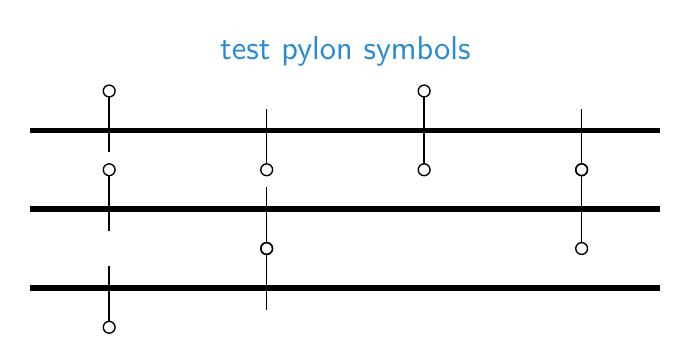
\begin{tikzpicture}[font=\sffamily]
    %!TEX TS-program = pdflatexmk
%!TEX root = test.tex

% Copyright (c) 2018 - 2022, Martin Scheidt (ISC license)
% Permission to use, copy, modify, and/or distribute this file for any purpose with or without fee is hereby granted, provided that the above copyright notice and this permission notice appear in all copies.

\node[blue] at (4,0) {\large test pylon symbols};

\foreach \i in {1,2,...,3}{
  \coordinate (A\i) at ($(0,0) + (0,-\i)$);% base coordinate
  \coordinate (B\i) at ($(8,0) + (0,-\i)$);% base coordinate
  %
  \maintrack (A\i) --   (B\i); % draw main tracks on base coordinate
  %
  % coordinates for testing symbols
  \coordinate (X\i-1) at ($(1,0) + (0,-\i)$);
  \coordinate (X\i-2) at ($(3,0) + (0,-\i)$);
  \coordinate (X\i-3) at ($(5,0) + (0,-\i)$);
  \coordinate (X\i-4) at ($(7,0) + (0,-\i)$);
}

\pylon[side=left ] at (X1-1);
\pylon[] at (X1-2);
\pylon[side=both ] at (X1-3);
\pylon[side=right] at (X1-4);
\pylon[side=left ] at (X2-1);
\pylon[side=right] at (X2-2);
\pylon[side=left ] at (X2-4);
\pylon[side=right] at (X2-4);
\pylon[side=right] at (X3-1);
\pylon[side=left ] at (X3-2);
  \end{tikzpicture}

  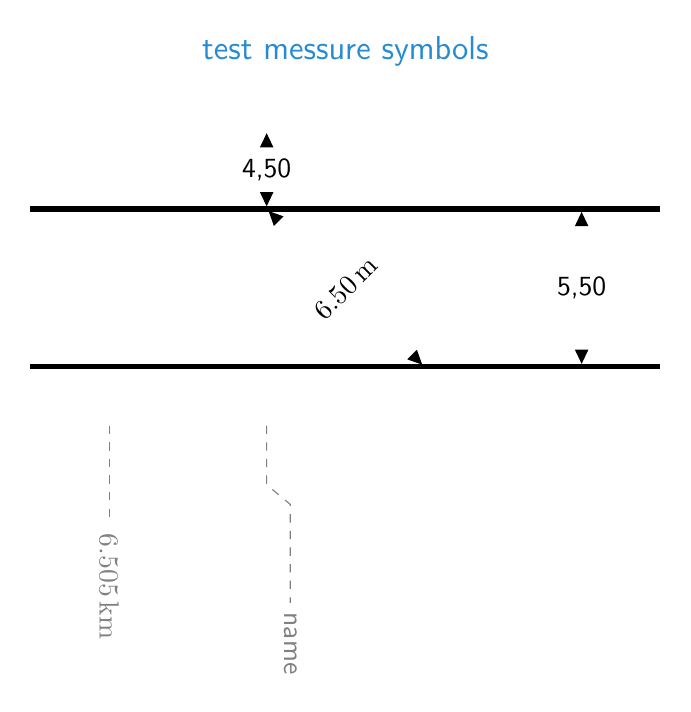
\begin{tikzpicture}[font=\sffamily]
    %!TEX TS-program = pdflatexmk
%!TEX root = test.tex

% Copyright (c) 2018 - 2022, Martin Scheidt (ISC license)
% Permission to use, copy, modify, and/or distribute this file for any purpose with or without fee is hereby granted, provided that the above copyright notice and this permission notice appear in all copies.

\node[blue] at (4,0) {\large test messure symbols};

\foreach \i in {1,2,3}{% base coordinate
  \coordinate (A\i) at ($(0,0) + 2*(0,-\i)$);% base coordinate
  \coordinate (B\i) at ($(8,0) + 2*(0,-\i)$);% base coordinate
}

\foreach \i in {1,2}{% draw main tracks on base coordinate
  \maintrack (A\i) --   (B\i);
}

\foreach \i in {1,2}{% coordinates for testing symbols
  \coordinate (X\i-1) at ($(1,0) + 2*(0,-\i)$);
  \coordinate (X\i-2) at ($(3,0) + 2*(0,-\i)$);
  \coordinate (X\i-3) at ($(5,0) + 2*(0,-\i)$);
  \coordinate (X\i-4) at ($(7,0) + 2*(0,-\i)$);
}

\trackdistance between (3,-1) and (X1-2) label (4,50);
\trackdistance between (X1-2) and (X2-3) label (\sffamily \SI{6,50}{\metre});
\trackdistance between (X1-4) and (X2-4) label (5,50);

\tikzset{hectometer base={(A3)},orientation=right};
\hectometer[] at (X2-1) mileage (\sffamily \SI{6,505}{\kilo\metre});
\hectometer[shift label={(0.3,-1)}] at (X2-2) mileage (name);
% \measureline between (a) and (b);
  \end{tikzpicture}
  
  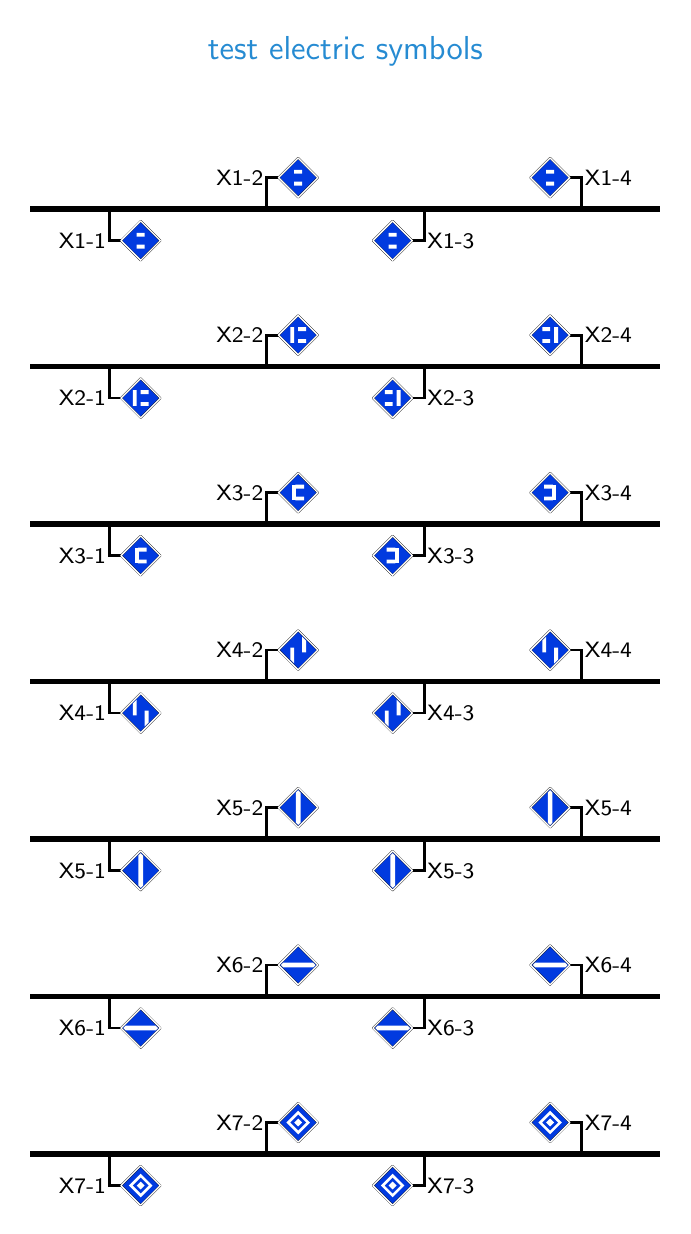
\begin{tikzpicture}[font=\sffamily]
    %!TEX TS-program = pdflatexmk
%!TEX root = test.tex

% Copyright (c) 2018 - 2022, Martin Scheidt (ISC license)
% Permission to use, copy, modify, and/or distribute this file for any purpose with or without fee is hereby granted, provided that the above copyright notice and this permission notice appear in all copies.

\node[blue] at (4,0) {\large test electric symbols};

\foreach \i in {1,2,...,7}{% base coordinate
  \coordinate (A\i) at ($(0,0) + 2*(0,-\i)$);% base coordinate
  \coordinate (B\i) at ($(8,0) + 2*(0,-\i)$);% base coordinate
  %
  \maintrack (A\i) --   (B\i); % draw main tracks on base coordinate
  %
  % coordinates for testing symbols
  \coordinate (X\i-1) at ($(1,0) + 2*(0,-\i)$);
  \coordinate (X\i-2) at ($(3,0) + 2*(0,-\i)$);
  \coordinate (X\i-3) at ($(5,0) + 2*(0,-\i)$);
  \coordinate (X\i-4) at ($(7,0) + 2*(0,-\i)$);
}

\distantpoweroff[forward ] at (X1-1) label (X1-1);
\distantpoweroff[forward ,position=left] at (X1-2) label (X1-2);
\distantpoweroff[backward,position=left] at (X1-3) label (X1-3);
\distantpoweroff[backward] at (X1-4) label (X1-4);

\poweroff[forward ] at (X2-1) label (X2-1);
\poweroff[forward ,position=left] at (X2-2) label (X2-2);
\poweroff[backward,position=left] at (X2-3) label (X2-3);
\poweroff[backward] at (X2-4) label (X2-4);

\poweron[forward ] at (X3-1) label (X3-1);
\poweron[forward ,position=left] at (X3-2) label (X3-2);
\poweron[backward,position=left] at (X3-3) label (X3-3);
\poweron[backward] at (X3-4) label (X3-4);

\distantpantographdown[forward ] at (X4-1) label (X4-1);
\distantpantographdown[forward ,position=left] at (X4-2) label (X4-2);
\distantpantographdown[backward,position=left] at (X4-3) label (X4-3);
\distantpantographdown[backward] at (X4-4) label (X4-4);

\pantographdown[forward ] at (X5-1) label (X5-1);
\pantographdown[forward ,position=left] at (X5-2) label (X5-2);
\pantographdown[backward,position=left] at (X5-3) label (X5-3);
\pantographdown[backward] at (X5-4) label (X5-4);

\pantographup[forward ] at (X6-1) label (X6-1);
\pantographup[forward ,position=left] at (X6-2) label (X6-2);
\pantographup[backward,position=left] at (X6-3) label (X6-3);
\pantographup[backward] at (X6-4) label (X6-4);

\wirelimit[forward ] at (X7-1) label (X7-1);
\wirelimit[forward ,position=left] at (X7-2) label (X7-2);
\wirelimit[backward,position=left] at (X7-3) label (X7-3);
\wirelimit[backward] at (X7-4) label (X7-4);

  \end{tikzpicture}
\end{document}